\documentclass{beamer}
\usepackage{graphicx}
\usepackage{paralist}
\usepackage{outlines}

\title{Eraser Tools}
\author{Mendocino College - Image Manipulation with Photoshop}
\titlegraphic{\vspace{-10mm}
\includegraphics[width = .8\textwidth]{images/photoshop.jpg}} 
\date{\vspace{-5em}} 


\mode <presentation>
\usetheme{Warsaw}
\usecolortheme{default}

\setbeamerfont{footline}{size=\fontsize{5}{8}\selectfont}

\definecolor{darkred}{rgb}{20,0,0}
\definecolor{darkgreen}{RGB}{40,110,20}
\definecolor{darkpurple}{RGB}{30,0,30}
\definecolor{chardonnay}{RGB}{255, 255, 204}

\setbeamercolor*{palette primary}{fg=white, bg=darkgreen}


\begin{document}
	{
		\setbeamertemplate{footline}{} 
		\setbeamertemplate{headline}{} 
		\begin{frame}
			\vspace{-35pt}
			\maketitle
		\end{frame}
	}

\section{What is the Eraser Tool?}	

\begin{frame}
	\frametitle{Eraser Tool}
	\begin{center}
		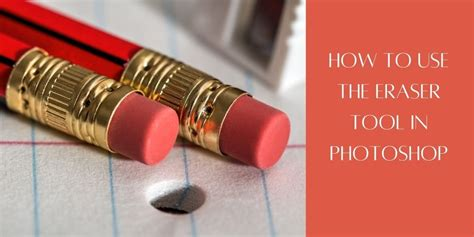
\includegraphics[width = 1.0\textwidth]{images/th (2).jpg}
	\end{center}
\end{frame}

\subsection{What is the Eraser Tool?}	
\begin{frame}
	\frametitle{What is the Eraser Tool?}
	\begin{outline}
		\1 In the options bar, choose a Mode setting. 
		\2 Brush and Pencil set the eraser to act like those tools. 
		\2 Block is a hard-edged, fixed-sized square with no options for changing the opacity or flow.
		\1 An opacity of 100\% erases pixels completely. A lower opacity erases pixels partially.
	\end{outline}
	\begin{center}
		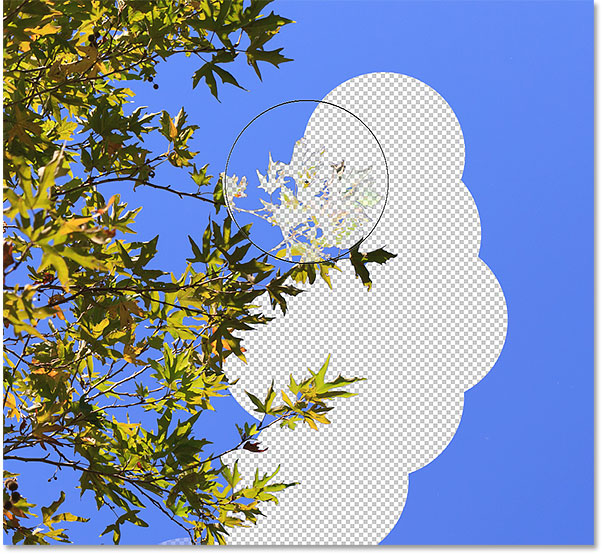
\includegraphics[width = 0.75\textwidth]{images/background-eraser-example-2.jpg}
	\end{center}
\end{frame}

\begin{frame}
	\frametitle{Eraser Tool Options}
	\begin{outline}
		\1 The Eraser tool changes pixels to either the background color or to transparent. 
		\1 If you’re working on a background (or in a layer with transparency locked), the pixels change to the background color; 
		\2 otherwise, the pixels are erased to transparency.
	\end{outline}
	\begin{center}
		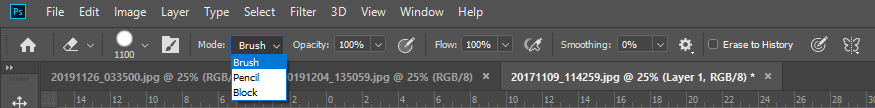
\includegraphics[width = 1.25\textwidth]{images/eraser modes.png}
	\end{center}
\end{frame}

	\section{Magic Eraser Tool}
	\subsection{Magic Eraser Tool}
\begin{frame}
	\frametitle{Magic Eraser Tool}
	\begin{outline}
		\1 When you click in a layer with the Magic Eraser tool, the tool changes all similar pixels to transparent. 
		\1 If you’re working in a layer with locked transparency, the pixels change to the background color. 
		\1 If you click in the background, it is converted to a layer and all similar pixels change to transparent.
		\1 You can choose to erase contiguous pixels only or all similar pixels on the current layer.
	\end{outline}
	\begin{center}
		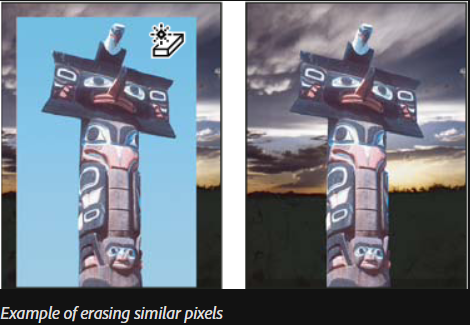
\includegraphics[width = 0.45\textwidth]{images/magic eraser.png}
	\end{center}
\end{frame}

	\subsection{Magic Eraser Tool - Options}
\begin{frame}
	\frametitle{Magic Eraser Tool - Options}
	\begin{outline}
		\1 Tolerance value: 
		\2 Defines the range of colors that can be erased. A low tolerance erases pixels within a range of color values very similar to the pixel you click. A high tolerance extends the range of colors that will be erased.
		\1 Select Anti-aliased to smooth the edges of the area you erase.
		\1 Select Contiguous to erase only pixels contiguous to the one you click, or deselect to erase all similar pixels in the image.
		\1 Select Sample All Layers to sample the erased color using combined data from all visible layers.
		\1 Specify an opacity to define the strength of the erasure. An opacity of 100\% erases pixels completely. A lower opacity erases pixels partially.
	\end{outline}
	\begin{center}
		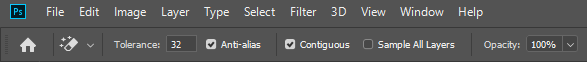
\includegraphics[width = 1.0\textwidth]{images/magic eraser 2.png}
	\end{center}
\end{frame}
	
	
	\section{Background Eraser Tool}
	\subsection{Background Eraser Tool}
	\begin{frame}
		\frametitle{Background Eraser Tool}
		\begin{outline}
			\1 Changes pixels on layer to transparent as you drag.
			\1 You can erase the background while maintaining the edges of an object in the foreground.
			\1 The background eraser samples the color in the center of the brush, also called the hotspot, and deletes that color wherever it appears inside the brush. 
			\1 It also performs color extraction at the edges of any foreground objects, so that color halos are not visible if the foreground object is later pasted into another image.
			\1 Note:  It overrides the lock transparency setting of a layer.
		\end{outline}
		\begin{center}
		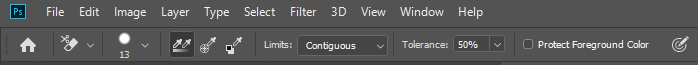
\includegraphics[width = 1.0\textwidth]{images/background eraser.png}
	\end{center}
	\end{frame}

	\subsection{Background Eraser Tool - Options}
	\begin{frame}
	\frametitle{Background Eraser Tool - Options}
	\begin{outline}
		\1 Choose a Limits mode for erasing: Discontiguous to erase the sampled color wherever it occurs under the brush; Contiguous to erase areas that contain the sampled color and are connected to one another; and Find Edges to erase connected areas containing the sampled color while better preserving the sharpness of shape edges.
		\1 For Tolerance, enter a value or drag the slider. A low tolerance limits erasure to areas that are very similar to the sampled color. A high tolerance erases a broader range of colors.
		\1 Select Protect Foreground Color to prevent the erasure of areas that match the foreground color in the toolbox.
		\1 Choose a Sampling option: Continuous to sample colors continuously as you drag; Once to erase only areas containing the color you first click; and Background Swatch to erase only areas containing the current background color.
	\end{outline}
\end{frame}


	\section{Auto Erase with the Pencil Tool}	

	\subsection{Auto Erase with the Pencil Tool}
	\begin{frame}
		\begin{outline}
			\1 The Auto Erase option for the Pencil tool lets you paint the background color over areas containing the foreground color.
			\1 Select the Pencil tool
			\2 Specify foreground and background colors.
			\2 Select Auto Erase in the options bar.
			\2 Drag over the image.
			\3 If the center of the cursor is over the foreground color when you begin dragging, the area is erased to the background color. If the center of the cursor is over an area that doesn’t contain the foreground color when you begin dragging, the area is painted with the foreground color.
\end{outline}
\begin{center}
	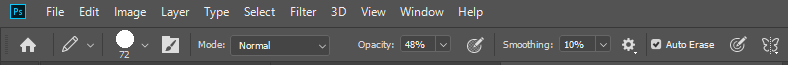
\includegraphics[width = 1.0\textwidth]{images/auto erase.png}
\end{center}
\end{frame}

\end{document}